%%%%%%%%%%%%%%%%%%%%%%%%%%%%%%%%%%%%%%%%%
% University/School Laboratory Report
% LaTeX Template
% Version 3.1 (25/3/14)
%
% This template has been downloaded from:
% http://www.LaTeXTemplates.com
%
% Original author:
% Linux and Unix Users Group at Virginia Tech Wiki 
% (https://vtluug.org/wiki/Example_LaTeX_chem_lab_report)
%
% License:
% CC BY-NC-SA 3.0 (http://creativecommons.org/licenses/by-nc-sa/3.0/)
%
%%%%%%%%%%%%%%%%%%%%%%%%%%%%%%%%%%%%%%%%%

%----------------------------------------------------------------------------------------
%	PACKAGES AND DOCUMENT CONFIGURATIONS
%----------------------------------------------------------------------------------------

\documentclass[a4paper]{article}

\usepackage[margin=1 in]{geometry}
\usepackage{listings}
\usepackage{graphicx} % Required for the inclusion of images
\usepackage{natbib} % Required to change bibliography style to APA
\usepackage{amsmath} % Required for some math elements 
\usepackage{hyperref}


\setlength\parindent{0pt} % Removes all indentation from paragraphs

%\renewcommand{\labelenumi}{\alph{enumi}.} % Make numbering in the enumerate environment by letter rather than number (e.g. section 6)


%----------------------------------------------------------------------------------------
%	DOCUMENT INFORMATION
%----------------------------------------------------------------------------------------

\title{Final project report on \\Path Finding Problem \\~ \\ CS 7750} % Title

\author{Chanmann Lim \\Zolbayar Magsar \\Yihan Xu}

\date{December 15, 2014}

\begin{document}

\maketitle % Insert the title, author and date

\lstset{language=Java,title=\lstname,basicstyle=\footnotesize}

\begin{center}
Computer Science Department \\
University of Missouri, Columbia \\
\vspace{.5 in}
Instructor: Dr. Yi Shang \\
\end{center}

\vspace{1 in}

% If you wish to include an abstract, uncomment the lines below
\begin{abstract}
In many occasions, we face the problem of finding a path from one place to another place. In such situations, were we not just trying to find the shortest distance; but the traveling time also an important factor to be taken into consideration. In artificial intelligence, search algorithms are mainly used for such problems. On the other hand, when it comes to differentiating between such algorithms, it is often useful to implement them on a path finding problem and compare their features. We have attempted to create a game map which can be used in a simple path finding problem. On the map, we have two points, start and destination. We are also free to create an arbitrary shape of walls between them to create a problem. We then have myriad of ways to examine the precise difference between search algorithms and compare them in terms of execution speed, accuracy, and overall performance. To solve the path finding problem, we have implemented six major search algorithms representing 3 main types of search algorithm families, namely Breadth-First Search, Depth-First Search, Greedy Best-First Search, A* Search, Hill-Climbing, and Simulated Annealing. The map is created using a grid structure, so as to have a precise depiction of the 'search movements' of each of the algorithms visually in terms of characteristics and performance.
\end{abstract}

% \vfill

%----------------------------------------------------------------------------------------
%	SECTION 1
%----------------------------------------------------------------------------------------

\section{Introduction}

Wikipedia describes the pathfinding problem as "\emph{Pathfinding} or \emph{pathing} is the plotting, by a computer application, of the shortest route between two points". There are two main problems of pathfinding, which are:

\begin{itemize}
	\item Finding a path between two nodes in a graph 
	\item Finding the optimal path
\end{itemize}

Blind search algorithms such as breadth-first and depth-first search solve the first type of problem by exhaustively checking all possibilities, starting with the given node. They iterate through all possible paths until they find the destination node. Because of their “blindness”, such algorithms can be either ineffective or too expensive. \\

Then we have an even more complicated problem – finding the optimal path. In this case however, it is not required to check all possible paths in order to find the optimal one. By using heuristics (additional knowledge of the problem space), we can strategically eliminate unnecessary paths. We will find out that this informed approach is more powerful and "gets the job done" efficiently most of the time. \\

We also have a type of search algorithms that try to explore the search space unsystematically. This is relative to the fact that, in some problems, the path to the goal is irrelevant – what matters is the final state after the search effort. Local search algorithms are such algorithms in which the paths followed are not retained. \\
 
We have implemented six different algorithms reflecting the above three different approaches: \\
\begin{itemize}
	\item Uninformed search
	\begin{itemize}
		\item Breadth-first search
		\item Depth-first search
	\end{itemize}

	\item Heuristic search
	\begin{itemize}
		\item Greedy best-first search
		\item A* search
	\end{itemize}

	\item Local search
	\begin{itemize}
		\item Hill-climbing search
		\item Simulated annealing
	\end{itemize}
\end{itemize}

% \subsection{Definitions}
% \label{definitions}
% \begin{description}
% \item[Stoichiometry]
% The relationship between the relative quantities of substances taking part in a reaction or forming a compound, typically a ratio of whole integers.
% \item[Atomic mass]
% The mass of an atom of a chemical element expressed in atomic mass units. It is approximately equivalent to the number of protons and neutrons in the atom (the mass number) or to the average number allowing for the relative abundances of different isotopes. 
% \end{description} 
 
%----------------------------------------------------------------------------------------
%	SECTION 2
%----------------------------------------------------------------------------------------

\section{Algorithms and Implementations}

There will be obstacles between the start and the destination squares, and our implementation shows graphically how each algorithm manage to reach the destination in its own term. This very activity will in turn allow us to visually enjoy the actual performance of each of those algorithms in real world problems. We made use of Manhattan distance heuristics for the informed search algorithms and as the scoring/objective function for local searches.

%----------------------------------------------------------------------------------------
%	Breadth-first
%----------------------------------------------------------------------------------------

\subsection{Breadth-first search algorithm:}

Breadth First search is known as an uninformed search because it does not use any information about how far it has traveled or how far it is from the goal. BFS begins at the starting position and looking for the goal by expanding all of the allowable directions of the root node from the order of left, up, right and down. All nodes that have already been visited, block nodes and nodes outside map will not be considered allowable nodes. \\

Breadth First Search follows a First in First out queue. Once the goal is found, it then trace back through the tree to obtain the path for the agent to follow. \\

\begin{figure}[h!]
  \centering
    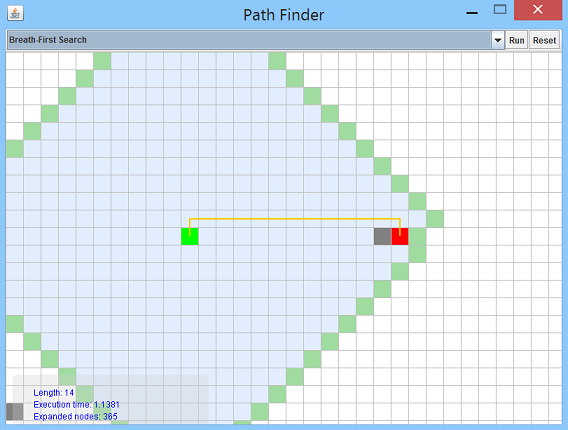
\includegraphics[scale=.9]{images/bfs1.png}
  \caption{BFS with a block between two points}
\end{figure}

The algorithm uses a queue data structure to store intermediate results as it traverses the graph, as follows:\\

\begin{enumerate}
\item Enqueue the root node
\item Dequeue a node in first-in-first-out manner and examine it
	\begin{itemize}
		\item If the element sought is found in this node, quit the search and return a result.
		\item Otherwise enqueue any successors (the direct child nodes) that have not yet been discovered.
	\end{itemize}
\item If the queue is empty, every node on the graph has been examined – quit the search and return "not found". \\
\item If the queue is not empty, repeat from Step 2.
\end{enumerate}

%----------------------------------------------------------------------------------------
%	Depth-first
%----------------------------------------------------------------------------------------

\subsection{Depth-first search algorithm:}

DFS starts at the root (selecting some arbitrary node as the root in the case of a graph) and explores as far as possible along each branch before backtracking. \\

\begin{figure}[h!]
  \centering
    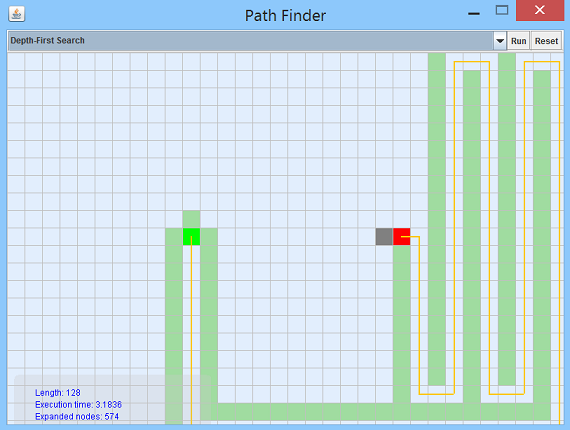
\includegraphics[scale=.9]{images/dfs1.png}
  \caption{DFS with a block between two points}
\end{figure}

DFS always expands the deepest node in the current frontier of the search tree. As seen above, the search proceeds immediately to the deepest level of the search tree, where the nodes have no successors.

%----------------------------------------------------------------------------------------
%	Greedy best-first
%----------------------------------------------------------------------------------------

\subsection{Best-first search algorithm:}

It is a search algorithm which explores a graph by expanding the most promising node chosen solely according to additional knowledge about the problem given by its designer in term heuristic function.\\

We used "best-first search" to refer specifically to a search with a heuristic function that attempts to predict how close the end of a path is to a solution, so that paths which are judged to be closer to a solution are extended first. This specific type of search is called \textbf{greedy best-first search}. \\

\begin{figure}[h!]
  \centering
    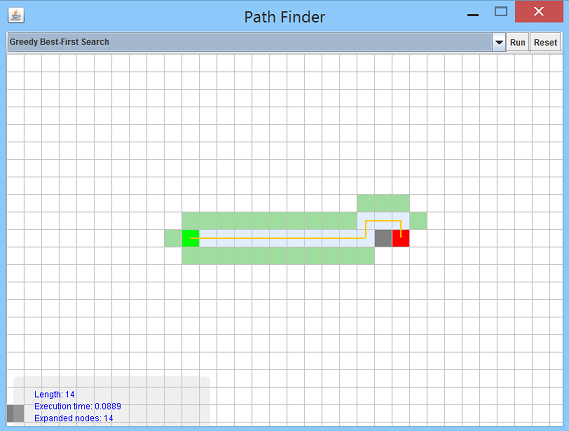
\includegraphics[scale=.9]{images/greedy1.png}
  \caption{Greedy best-first search with a block between two points}
\end{figure}

By using a greedy algorithm, we expand the root and add its successors to the queue then pick the successor that is the closest to the goal node depend entirely on the prediction of the heuristic function.

\paragraph{Manhattan distance heuristic: } Think of the grid map, the root node, and goal node in our PathFinding program as a cartesian plane with two separate points $x$ and $y$. What is your best estimate about the distance from $x$ to $y$? One might give the straight-line distance (euclidean distance) estimate however the sum of the difference between $x$ and $y$ coordinates (manhattan distance) would yield a more admissible prediction and in fact it is the perfect estimate as we define our grid to allow only horizontal and vertical move but not diagonal or straight a cross every square.  

%----------------------------------------------------------------------------------------
%	A*
%----------------------------------------------------------------------------------------

\subsection{A* search algorithm:}

\begin{figure}[h!]
  \centering
    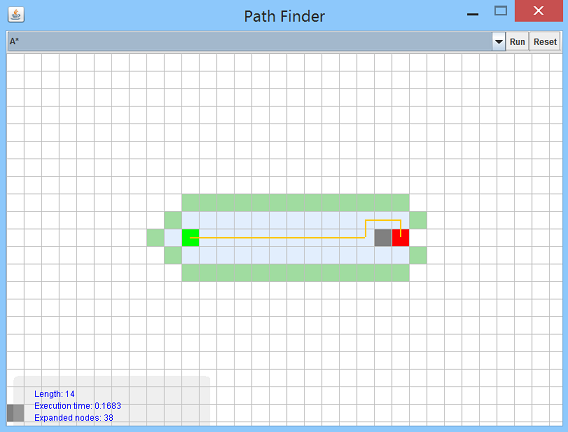
\includegraphics[scale=.9]{images/A1.png}
  \caption{A* with a block between two points}
\end{figure}

As compared to the Best-first search algorithm, A* explores a graph not only by expanding the most promising node based on the heuristic function, but also on take into account the cost to reach that intermediate node itself. We made use of the Manhattan distance heuristic function with A* search. Since Manhattan distance is a consistent heuristic, we are guaranteed to find an optimal path in case of A*. \\

The key difference from the implementation of Best-first search is that we keep a sorted priority queue (fringe) of alternate path segments in case of A*. Therefore, at each step, we remove the node with the lowest $f(x)$ value from the queue until reaching a goal square.

%----------------------------------------------------------------------------------------
%	Hill-climbing
%----------------------------------------------------------------------------------------

\subsection{Hill-climbing algorithm:}

As a local search algorithm, hill-climbing starts by exploring its neighbors and pick a candidate with the highest value evaluated by its objective function ($Manhattan\_distance * -1$) then compare the value of the neighbor node with its current node. If the neighbor node has a higher value the neighbor becomes the current node and repeat, otherwise it will exit the explore and compare loop, stop search and return a solution if the current node is the goal or failure if it is not. This often leads to improvement in search speed since it embraces the goal to always find a higher value neighboring square compare to its own without wasting time considering the currently poorer options and as a consequence it will get stuck on a locally optimal point. \\

\begin{figure}[h!]
  \centering
    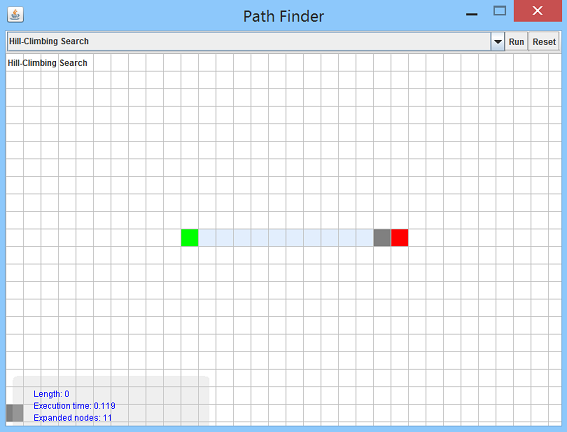
\includegraphics[scale=.9]{images/hillclimb1.png}
  \caption{Hill-climbing search with a block between two points}
  \label{fig:hillClimbing}
\end{figure}

Hence, in our grid map if there is an obstacle lying on the path to the goal node, the steepest-ascent hill-climbing we have implemented here will stop immediately as seen in the Figure~\ref{fig:hillClimbing}.

%----------------------------------------------------------------------------------------
%	Simulated annealing
%----------------------------------------------------------------------------------------

\subsection{Simulated annealing algorithm:}

Taking the advantage of search speech by not looking far ahead while trying to address the problem of getting stuck in local optima of a typical hill-climbing, simulated annealing starts by choosing a random successor and move to the square if it has a higher value than current position. Otherwise, accept the move only when the probability ($e^{\Delta E/T}$) is greater than a pseudorandomly generated number between $[0, 1]$. At the start, $T$ the temperature was initialized to $1000$ and the cooling schedule gradually decreases the temperature $T$ in each time step until $0$ and the search terminates if the goal hasn't been found. As temperature is getting lower the "bad" moves are becoming more unlikely driving the search to consider the moves more promising toward reaching the goal. \\

\begin{figure}[h!]
  \centering
    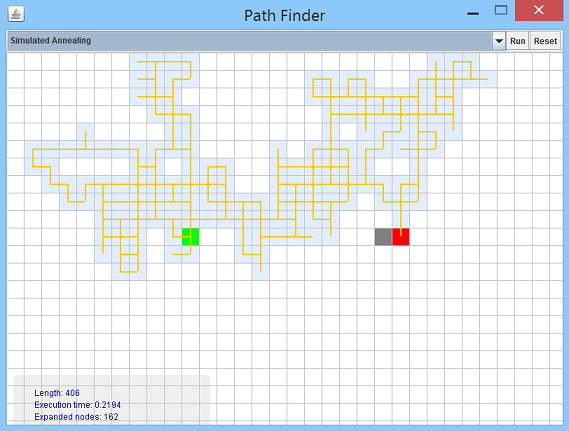
\includegraphics[scale=.9]{images/sa1.png}
  \caption{Simulated annealing with a block between two points}
  \label{fig:simulatedAnnealing}
\end{figure}

\paragraph{Cooling schedule:} Due to the randomness in picking a move with probability simulated annealing can manage to overcome local optima however in the hope to always reach the goal it very depends on the cooling schedule implementation. When the temperature decays too fast it will not be able to find the goal, but when the temperature decaying rate is too low the algorithm will take too many unnecessary trial and error moves and if there is no way to get to the goal node this exhaustive loop will still carry on as long as the temperature is greater than zero. Hence choosing the right cooling schedule function and its parameter is crucial to determine the productivity of the algorithm and the varying in size and characteristics of the problem space directly affect the decision to be made. In our situation, we use Linear Multiplicative Monotonic function \\

\begin{equation} \label{eq:linearMultiplicative}
T_k = \frac{T_0}{1 + \alpha \cdot k}, \quad \alpha > 0
\end{equation}
\\
where we set $T_0 = 1000$ and $\alpha = 0.1$, so the maximum loop here is 9991 for our simulated annealing algorithm. You can easily solve for $\alpha$ by tweaking the equation~\ref{eq:linearMultiplicative} to be \\

\begin{equation}
\alpha = \left(T_0-1\right) \cdot \frac{1}{k-1}
\end{equation}
\\
where $k$ is the maximum loop for your simulated annealing algorithm. \\

In term of Multiplicative cooling function, there are 3 other available choices including Exponential multiplicative cooling, Logarithmical multiplicative cooling, and Quadratic multiplicative cooling all of which not only consume more computational resource comparing to the linear function we are using but predictable nature of linearity also allows us to fine tune for an optimal $\alpha$ given discrete state space like our $22 \times 32$ grid map. \\

\begin{figure}[h!]
  \centering
    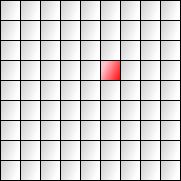
\includegraphics[scale=.6]{images/square-grid.png}
  \caption{Square grids}
\end{figure}

\paragraph{Use of grids:} Grids are widely used in games to represent a playground such as maps (Warcraft), playing surfaces (pool, tennis, poker), playing fields (baseball, football), boards (chess, Monopoly, Connect Four), and abstract spaces (Tetris). \\

We build grids by repeating simple shapes. A square grid is the most common type. It is the simplest type and very easy to work with, therefore the most common type of grid. We can represent locations using simple coordinates (x, y) system. The square coordinate system is the same even if your map squares are angled on screen in an isometric or axonometric projection. The default choice of heuristic function on a grid is understandably Manhattan distance heuristics, because of its block-type structure.

%----------------------------------------------------------------------------------------
%	SECTION 3
%----------------------------------------------------------------------------------------

\section{Results and Analysis}

The results we have obtained, after running these algorithms individually both with and without a block between the points A and B, are pretty astonishing and is a pleasure for anyone to watch how these algorithms get the job done through such distinctive methodologies.\\

\begin{figure}[h!]
  \centering
    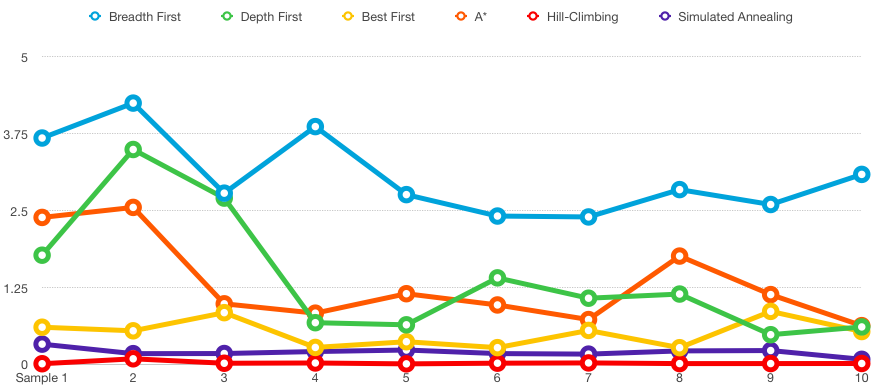
\includegraphics[scale=.4]{images/execution_time.png}
  \caption{Execution time comparison}
\end{figure}

As we can see in the chart, Breath First search takes more time than other algorithms for it needs more time to get an optimal path. Best first Search and A* Search, while they use heuristic to speed up the process and among which A* can still find optimal solution. Simulated annealing search and Hill-Climbing search take less time, among which Hill-Climbing search will stop very soon when it meets a local maxima. \\

\begin{figure}[h!]
  \centering
    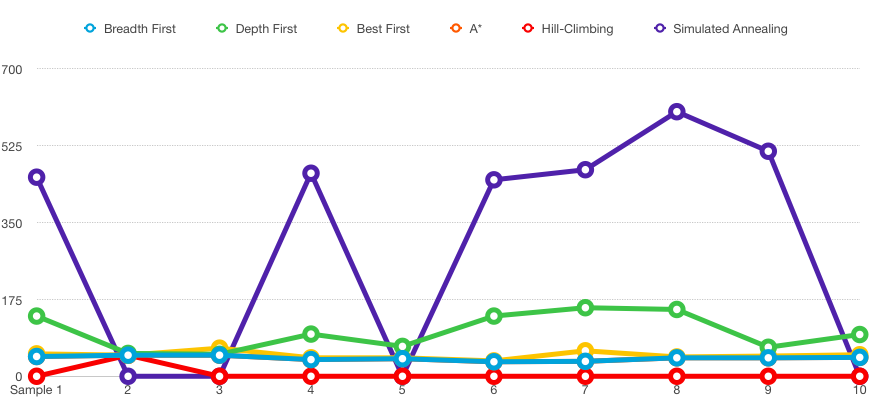
\includegraphics[scale=.4]{images/path_cost.png}
  \caption{Path cost comparison}
\end{figure}

As we can see in the chart above, Simulated Annealing search usually cost much more steps to reach the goal and sometimes even fail to reach the goal according to the cooling speed we set. Depth First Search cannot find an optimal solution while Breath First Search and A* Search can. Best First Search finds nearly as good as Breadth First Search and A* Search. \\

\begin{figure}[h!]
  \centering
    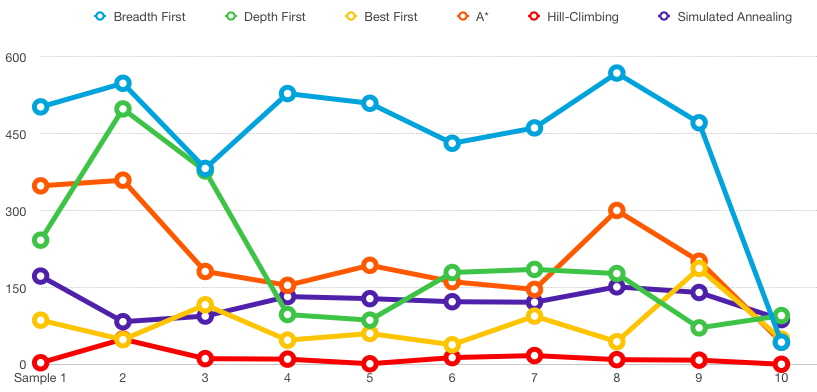
\includegraphics[scale=.4]{images/expanded_node.png}
  \caption{Expanded nodes comparison}
\end{figure}

As we can see in the chart above, Breath First Search and Depth First Search expanded the most amounts of nodes for they do not have heuristic function and will search all the way down to the goal.  The nodes expansion of A* Search, Best First Search and Simulated Annealing Search expands are very likely. \\



%----------------------------------------------------------------------------------------
%	SECTION 4
%----------------------------------------------------------------------------------------

\section{Conclusion}

So the obvious question is "which algorithm should we use for finding paths on a game map?"

\begin{itemize}
\item If you want to find paths from or to all locations, use Breadth First Search.
\item If you want to find paths to one location, use Greedy Best First Search or A*. We would prefer A* in most cases since it is optimal.
\end{itemize}

What about optimal paths? Breadth First Search is guaranteed to find the shortest path given the input graph. Greedy Best First Search is not. A* is guaranteed to find the shortest path if the heuristic is never larger than the true distance. As the heuristic becomes larger, A* turns into Greedy Best First Search.\\

What about performance? The best thing to do is to eliminate unnecessary locations in your graph. Reducing the size of the graph helps all the graph search algorithms. It also can be noticed that simpler queues run faster. Greedy Best First Search typically runs faster but doesn’t produce optimal paths. A* is a good choice for most pathfinding needs. \\

%----------------------------------------------------------------------------------------
%	SECTION 4
%----------------------------------------------------------------------------------------

\section{Source code}

\url{https://github.com/lchanmann/PathFinding}

\vfill

%----------------------------------------------------------------------------------------
%	BIBLIOGRAPHY
%----------------------------------------------------------------------------------------

\bibliographystyle{apalike}

\nocite{*}

\bibliography{ref}


%----------------------------------------------------------------------------------------


\end{document}